\documentclass[a4paper,10pt]{article}

\usepackage[T1]{fontenc}
\usepackage[utf8]{inputenc}
\usepackage{graphicx}
\usepackage{xcolor}
\usepackage{fourier}
\usepackage{caption}
\usepackage{subcaption}
\usepackage{cprotect}
\usepackage{tgtermes}

\usepackage[
pdftitle={Computer Aided Diagnosis}, 
pdfauthor={Luc Nies, Tom van de Poll, Harmen Prins, Steven Reitsma \& Inez Wijnands, Radboud University Nijmegen},
colorlinks=true,linkcolor=blue,urlcolor=blue,citecolor=blue,bookmarks=true,bookmarksopenlevel=2]{hyperref}
\usepackage{amsmath,amssymb,amsthm,textcomp}
\usepackage{enumerate}
\usepackage{multicol}
\usepackage{tikz}

\usepackage{geometry}
\geometry{total={210mm,297mm},
left=25mm,right=25mm,%
bindingoffset=0mm, top=20mm,bottom=20mm}

\numberwithin{equation}{section} % Number equations within sections (i.e. 1.1 instead of 1)
\numberwithin{figure}{section} % Number figures within sections (i.e. 1.1 i/o 1)
\numberwithin{table}{section} % Number tables within sections (i.e. 1.1 i/of 1)

\linespread{1.1}

\newcommand{\linia}{\rule{\linewidth}{0.5pt}}

% my own titles
\makeatletter
\renewcommand{\maketitle}{
\begin{center}
\vspace{2ex}
{\huge \textsc{\@title}}
\vspace{1ex}
\\
\linia\\
\@author  \@date
\vspace{4ex}
\end{center}
}
\makeatother

% custom footers and headers
\usepackage{fancyhdr,lastpage}
\pagestyle{fancy}
\lhead{}
\chead{}
\rhead{}
\lfoot{Phase \textnumero{} 1}
\cfoot{}
\rfoot{Page \thepage\ /\ \pageref*{LastPage}}
\renewcommand{\headrulewidth}{0pt}
\renewcommand{\footrulewidth}{0pt}

% code listing settings
\usepackage{listings}
\lstset{
    language=Python,
    basicstyle=\ttfamily\small,
    aboveskip={0.9\baselineskip},
    belowskip={0.9\baselineskip},
    columns=fixed,
    extendedchars=true,
    breaklines=true,
    tabsize=4,
    prebreak=\raisebox{0ex}[0ex][0ex]{\ensuremath{\hookleftarrow}},
    frame=lines,
    showtabs=false,
    showspaces=false,
    showstringspaces=false,
    keywordstyle=\color[rgb]{0.1,0.126,0.941},
    commentstyle=\color[rgb]{0.133,0.545,0.133},
    stringstyle=\color[rgb]{0,0.5,0},
    numbers=left,
    numberstyle=\scriptsize\ttfamily,
    stepnumber=1,
    numbersep=10pt,
    captionpos=t,
    escapeinside={\%*}{*)}
}

%%%----------%%%----------%%%----------%%%----------%%%

\begin{document}

\title{Computer Aided Diagnosis \\\vspace{0.2cm} Lung segmentation}

\author{Luc Nies (s4136748), Tom van de Poll (s4106512), Harmen Prins (s4132297),\\ Steven Reitsma (s4132343) \& Inez Wijnands (s4149696)\\ Radboud University Nijmegen\\}

\date{11/05/2016}

\maketitle

\section{Problem description}

\section{Fully convolutional network}

Since deep learning for image classification has emerged as an extremely successful method, other applications for deep learning have been explored.
One of these applications is image segmentation.
Long et al. \cite{long2015fully} propose a relatively simple method for using a convolutional neural network for image segmentation.
One of the challenges is that the output `label' of the classification is not a simple scalar label but is of the same dimensions as the input.
Another challenge is that the process of pixel-by-pixel classification is too slow for big datasets such as the one we are using.
Long et al. \cite{long2015fully} overcome both challenges with their method of using fully-convolutional networks for image segmentation.

During training time, we use 64x64 pixel patches that are extracted from slices in the horizontal plane of the image.
We assign a single label to the patch, defined by the class of the center pixel of the batch (either 0 for background or 1 for lung).
The network is fully-convolutional. This means that no fully-connected layers are used, only convolutional and pooling layers.
This is done so that images of various sizes can be used as input of the network.
If an image is inputed that has a size larger than 64x64 pixels, the result from the final layer in the network will be multidimensional in the spatial dimensions instead of a single label prediction.
This means that we can use our complete to-be-segmented image as the input of the trained network and the result will be a downsampled segmentation mask.
Of course, we need a normal-sized segmentation mask instead of a downsampled one.
To overcome the downsampling we use the shift-and-stitch method, also proposed by Long et al. \cite{long2015fully}.
---- HARMEN SHIFT N STITCH ----

Currently we have no results yet for the fully convolutional network as we are still in the development phase. However, the fully convolutional network can also be used for the next phase of the LUNA challenge (nodule candidate detection), by viewing is as a segmentation problem (we're trying to segment the candidates from the rest of the image). We are therefore continuing the development of this method and are confident that we will get it to work soon.

\section{Region growing in MeVisLab}
We used a second approach for segmenting the lungs from the CT scans which is the more conventional approach of using region growing, in order to compare the results of our FCN with the current `standard'. The biggest challenge of this approach is that in order to use region growing for segmentation, seed points need to be automatically selected inside the area that needs to be segmented. Since this is a difficult task, we circumvent this problem by using region growing in a different way. The following algorithm is used for segmentation:

\begin{itemize}
\item Threshold the image with threshold value 1000.
\item Apply region growing to the image, four times, with a corner pixel of the first slice as seed point.
\item Add the resulting four images to the thresholded image.
\item Threshold the resulting image with value 1000. An example result can be seen in figure \ref{fig:reg-gro}.
\item Invert the resulting image. All that is left are the lungs and some other artifacts. An example can be seen in figure \ref{fig:lung-meuk}.
\item Do a connected components analysis on the resulting image, and select only the largest component from the image (the lungs).
\item Since there are still black holes in the lungs (veins), closing is applied to the image with a 10x10x1 spherical kernel. An example of the resulting segmentation mask can be seen in figure \ref{fig:lungs}.
\end{itemize}

\noindent This approach circumvents the need to find specific region growing seed points, since we take the same seed points for each image, namely the four corner pixels of the first slice. The results gathered with this method seem fairly promising. More on the results of using this segmentation method is discussed in the section \ref{sec:results}.


\section{Results}
\label{sec:results}

\section{Conclusion}

\appendix
\section{Contributions}

\textbf{Luc Nies:}
\\
\textbf{Steven Reitsma:} Looked into implementing U-net. Afterwards assisted in getting the fully convolutional network to train. Wrote report section on fully convolutional networks.
\\
\textbf{Harmen Prins:}
\\
\textbf{Inez Wijnands:} Contributed to the initial implementation of the fully convolutional network. Contributed to creating the MeVisLab segmentation method. Implemented the evaluation method for the segmentations (Dice score).\\
\\
\textbf{Tom van de Poll:} Contributed to the initial implementation of the fully convolutional network. Contributed to creating the MeVisLab segmentation method and responsible for troubleshooting this method. Implemented the method for looping the MeVisLab segmentation method over the data.

\section{Figures}
\begin{figure}[h]
	\centering
	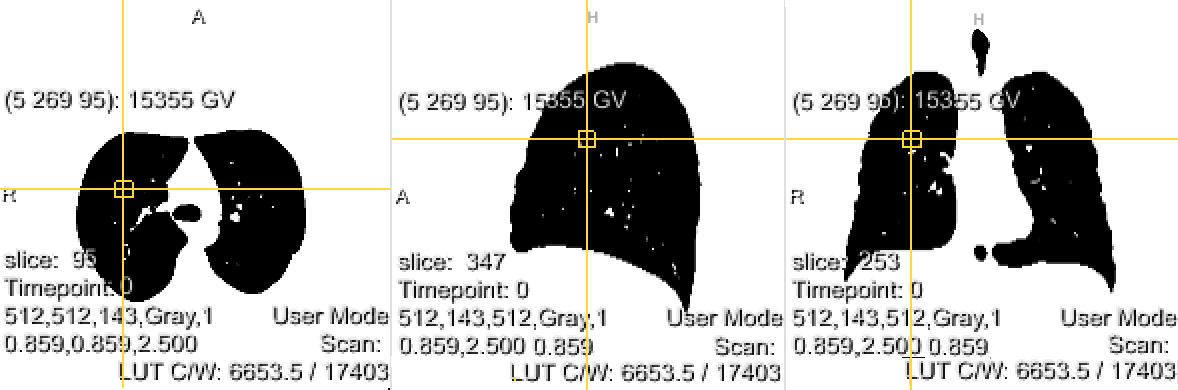
\includegraphics[scale=0.7]{regiongrowing}
    \caption{The thresholded image after region growing.}
    \label{fig:reg-gro}
\end{figure}

\begin{figure}[h]
    ~ %add desired spacing between images, e. g. ~, \quad, \qquad, \hfill etc. 
      %(or a blank line to force the subfigure onto a new line)
    \begin{subfigure}[b]{0.45\textwidth}
        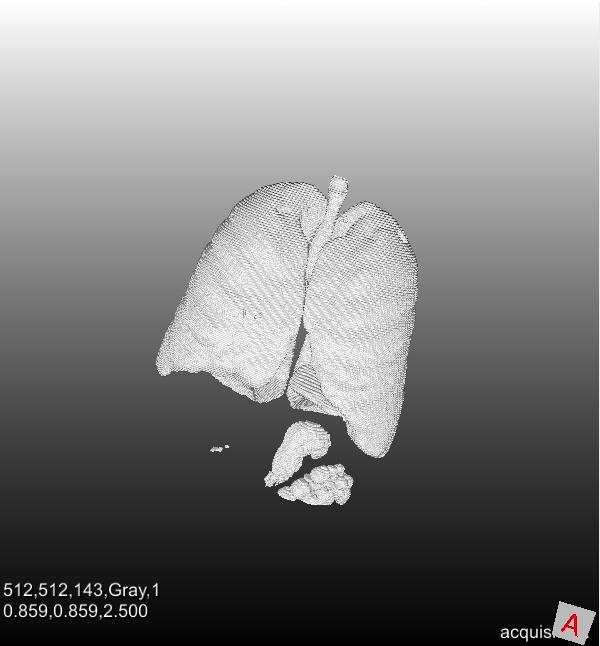
\includegraphics[width=\textwidth]{lungs_with_meuk}
        \caption{After the inversion step.}
        \label{fig:lung-meuk}
    \end{subfigure}
    ~ %add desired spacing between images, e. g. ~, \quad, \qquad, \hfill etc. 
    %(or a blank line to force the subfigure onto a new line)
    \begin{subfigure}[b]{0.45\textwidth}
        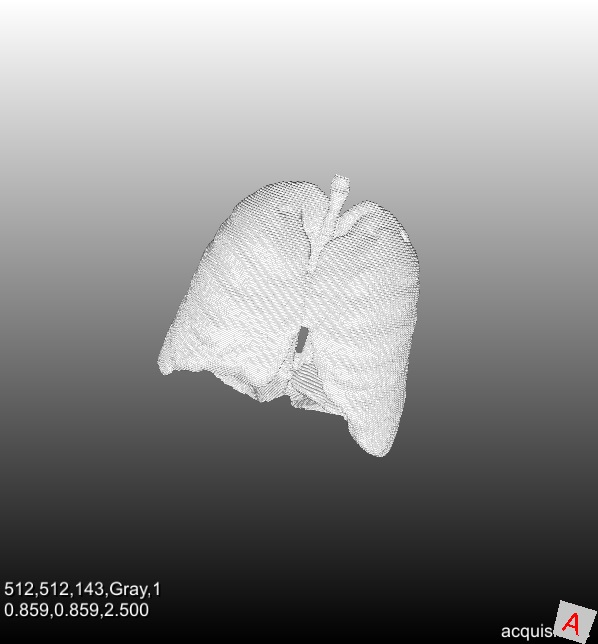
\includegraphics[width=\textwidth]{lungs_without_meuk}
        \caption{After connected component analysis and closing.}
        \label{fig:lungs}
    \end{subfigure}
    \caption{Results of the segmentation}\label{fig:lung-segmentation}
\end{figure}


\bibliographystyle{amsplain}
\bibliography{references}

\end{document}